% !TEX root = MAIN.tex

\chapter{Applicability to Space Software Standards}

To discuss applicability of mutation analysis and testing (either code-driven or data-driven) to different test levels (i.e., unit, integration, system, acceptance), we provide a generic overview of the interactions typically stressed by different test levels. Unit test cases focus on interactions within single units (e.g., functions belonging to a same source files) or few units belonging to a same component. Integration test cases trigger interactions between distinct units or multiple components. System test cases exercise interactions between all the components of the system.
Figure~\ref{fig:mutationTestingVSTestingLevels} provides a generic overview of the interactions typically stressed by different test levels

According to ECSS standards, system test cases might be executed on a host system with emulated hardware. Acceptance test cases exercise all the system components but in the operational environment. For this reason, mutation analysis/testing cannot be adopted in the context of acceptance testing because the deployment of multiple version of the system (one for each mutant) might be particularly expensive and may lead to safety hazards.
 
 
\begin{figure}[h]
  \centering
    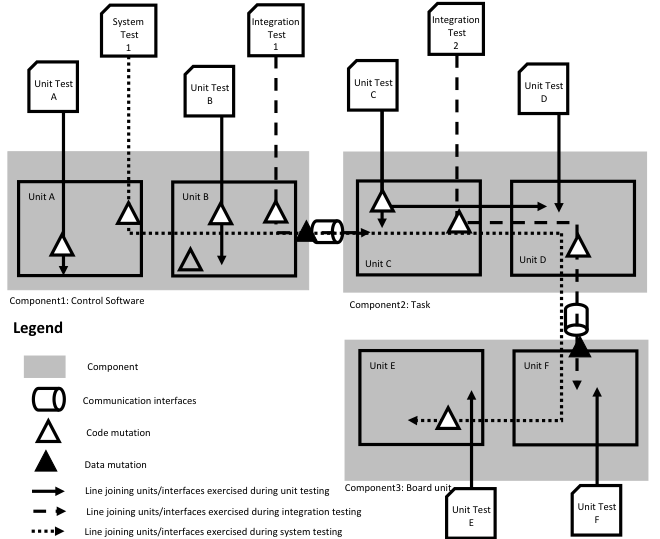
\includegraphics[width=10cm]{images/TestingLevels}
      \caption{Mutation Testing Approaches for Different Testing Levels.}
      \label{fig:mutationTestingVSTestingLevels}
\end{figure} 

%Test suite evaluation through code-driven mutation testing appear to be feasible for all the testing levels (i.e., unit, integration, and system), except acceptance testing for the reasons mentioned above. 

\INDEX{Unit testing} is the typical scenario in which code-driven mutation analysis and testing is adopted in other contexts, for this reason it should be targeted also in the case of space software.
In addition, code-driven test generation approaches based on static program analysis can be adopted to automatically generate unit test cases.
Data-driven mutation techniques, instead, are unlikely to be useful in the context of unit testing.
Indeed, Unit test cases do not verify the interaction between units but rely on stubs when the testing of a unit requires the interaction with another component.
% Also, although certain units focus on the communication with hardware components (e.g., chips) applying data-driven mutation techniques in that context would simply lead to a form of robustness testing targeting hardware components.

FAQAS has also shown that code-driven mutation analysis is feasible also in the context of \INDEX{integration testing} and \INDEX{system testing}. Code-driven test generation, instead, is not feasible in such contexts.

Integration and system test suite should also be the target of data-driven mutation analysis, which enables determining if relevant scenarios had been exercised (i.e., scenarios where all the possible message exchanges had been covered). 


Depending on the development process, system-level test cases may focus only on specific features of the system under test; while unit test cases might be used only to cover exceptional cases. For this reason, each of these test suite may not reach 100\% statement coverage. For the same reason, they may kill distinct subsets the mutants generated for the system. 
We suggest to compute the mutation score by considering all the available test suites (i.e., a mutant is killed if at least one test case of any available test suite fails).

\begin{figure}[h]
  \centering
    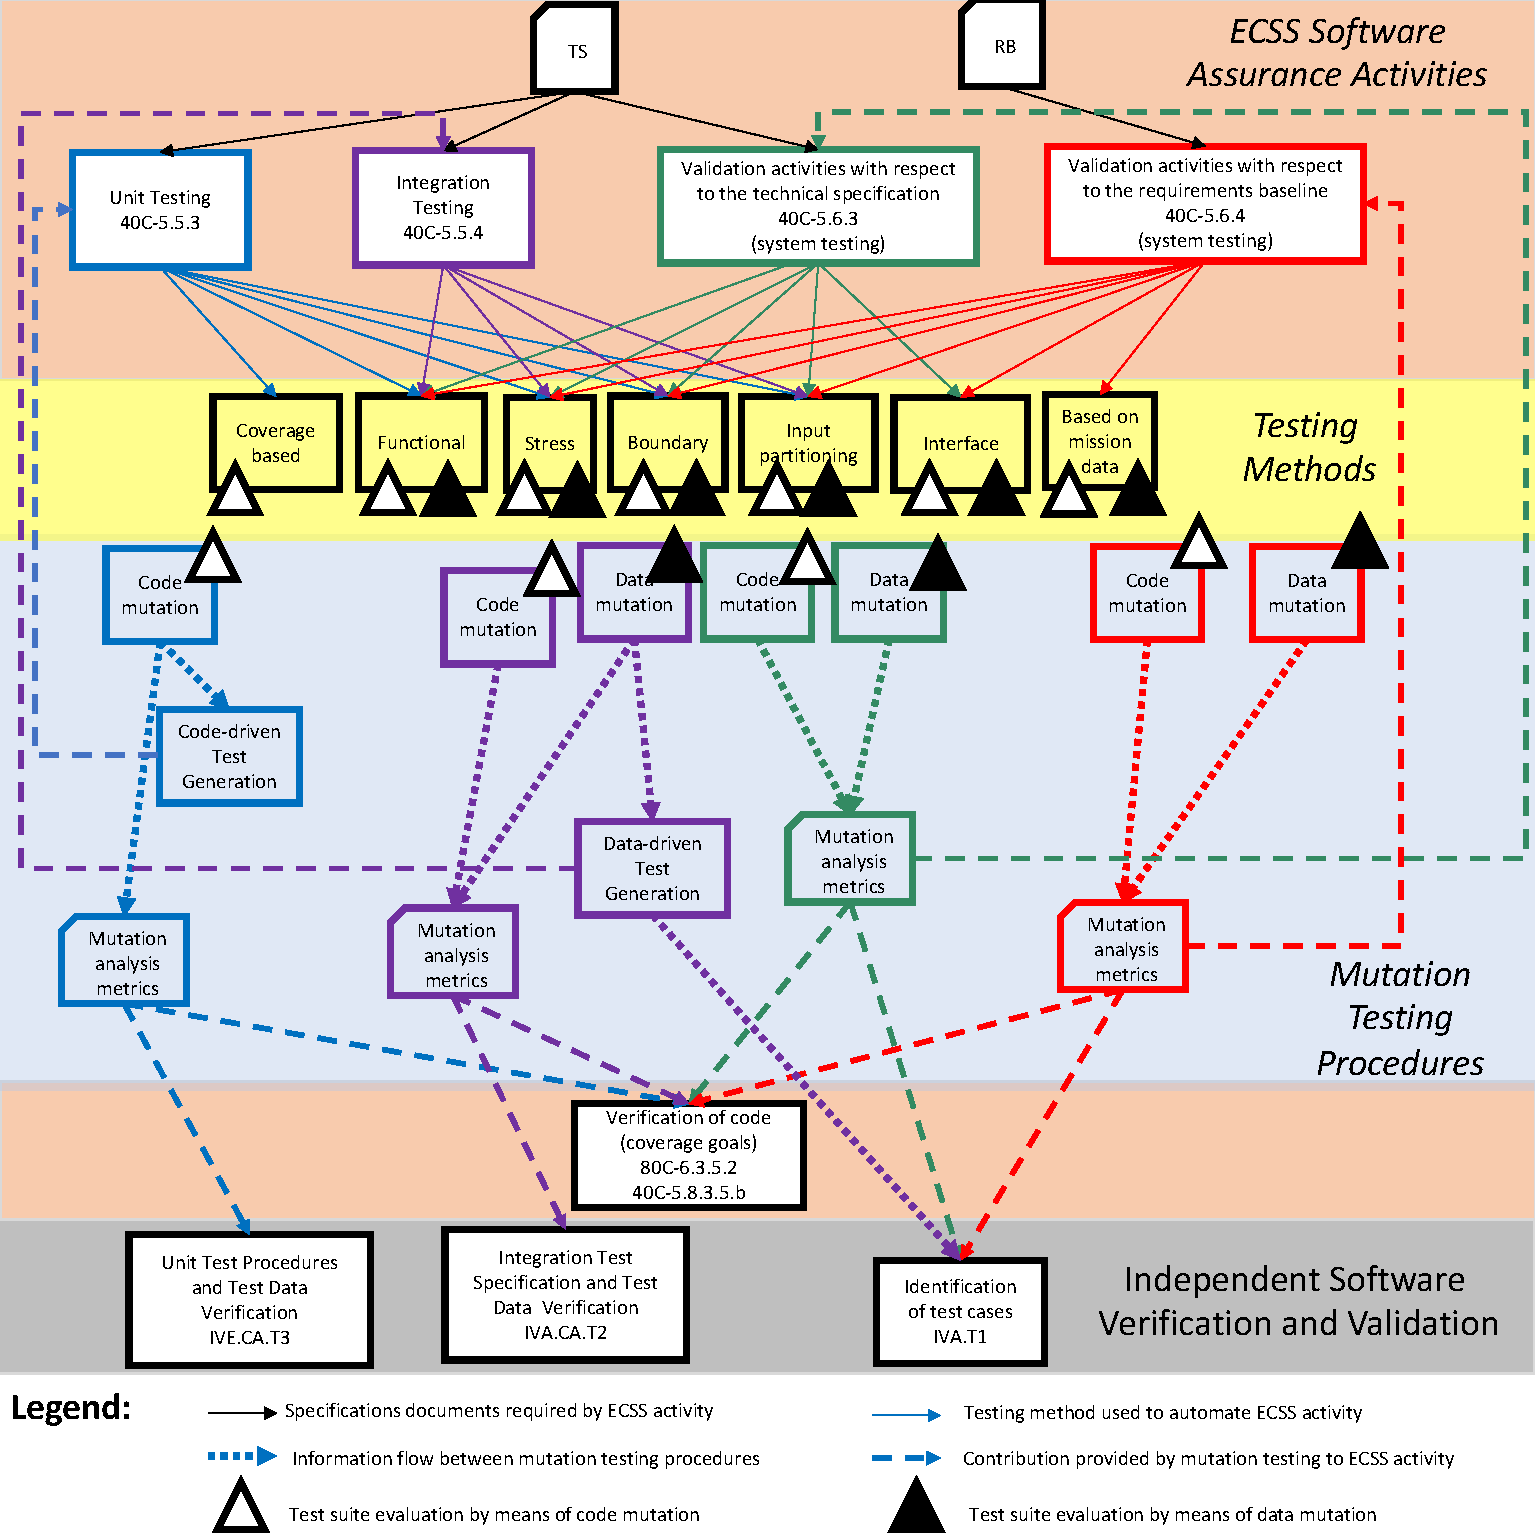
\includegraphics[width=0.9\textwidth]{images/ECSSTesting}
      \caption{Relations between ECSS activities and activities of the mutation testing process.}
      \label{fig:ECSSTesting}
\end{figure} 

Figure~\ref{fig:ECSSTesting} shows the relationships between ECSS software testing practices and the main activities of the mutation analysis/testing process: code mutation, data mutation, code-driven test generation (SEMuS), data-driven test generation (DAMTE), and inspection of mutation analysis metrics (to either evaluate test suite or derive test cases manually. These relationships guide the definition of a mutation testing process integrated with ECSS standards.
 
In Figure~\ref{fig:ECSSTesting}, black arrows show the specifications documents (i.e., Technical Specifications and Requirement Baselines) used to support ECSS testing activities (i.e., Unit Testing, Integration Testing, Validation activities with respect to the technical specification and Validation activities with respect to the requirements baselines). Colored arrows are used to associate ECSS activities to specific testing methods suggested in the ECSS standard (e.g., mission data is used for ECSS-E-ST-40C-5.6.4). Triangles are used to indicate which type of mutation testing (i.e., code-driven or data-driven) is likely applicable when a specific testing method is applied. White triangles are used to indicate that code mutation can be applied with a certain testing method, black triangles are used for data mutation. 

Concerning the type of mutation activity associated to each testing method, we observe that code-driven mutation might be used for all the testing methods in use; sampling strategies will help code-driven mutation scale in the presence of long executions. Data-driven mutation, instead, is unlikely to be used with coverage based testing which often targets unit tests. 

Test case generation based on symbolic execution can be used in the context of unit testing targeted by code-driven mutation (with SEMuS) and in the context of integration testing targeted by data-driven mutation (with DAMTE applied in the presence of specific architectures). For code-driven mutation, integration test suites can be improved only manually (because of the limitations of KLEE). System test suites can be improved only manually.

In Figure~\ref{fig:ECSSTesting}, dashed arrows show how the mutation testing procedures can contribute to ECSS activities. 
Overall, mutation analysis can be used to verify UT/IT/TS-RB test suites and guide engineers towards improving them (e.g., by selecting test inputs to kill mutants). Mutation testing may support the generation of unit test cases. Such support might be provided in both software (SW) and ISVV life cycles. 
The mutation analysis metrics (e.g., mutation score) might be used to support SW verification activities; more precisely, they might be used as an additional coverage metric for the activities described in ECSS-Q-ST-80C 6.3.5.2 and ECSS-E-ST-40C 5.8.3.5.b. Also, mutation testing (i.e., automated test generation) supports the improvement of test sites. Independent Software Verification and Validation~\cite{ESAISVV} can benefit from the mutation analysis/testing process as well. The mutation analysis metrics can support Unit Test Procedures and Test Data Verification (IVE.CA.T3 in~\cite{ESAISVV}) and Integration Test Specification and Test Data Verification (IVA.CA.T2 in~\cite{ESAISVV}). Finally, test generation and mutation score may support ISVV during the identification of test cases (IVA.T1 in~\cite{ESAISVV}).
